\chapter{Grensvlakken, oppervlakteactieve stoffen en colloïden}\label{ch:b3:colloids}

Mayonaise is olie, verdeeld in druppeltjes van enkele micrometer in een
beetje water en azijn, en uit elkaar gehouden door het lecithine en de
eiwitten van eigeel. Wie in het begin te snel klopt of de olie te snel
toevoegt, ziet ze schiften in een olieachtige en een waterige laag: de
druppels versmelten en de energie die ze uit elkaar hield, is weg. Melk,
mist, inkt, verf, bloed en het modderige water van een rivier zijn
materie van dezelfde soort: deeltjes of druppels die veel groter zijn dan
moleculen en veel kleiner dan wat het oog ziet, en zo talrijk dat de
meeste van hun moleculen dicht bij een grensvlak liggen. Dit hoofdstuk
behandelt de energie van grensvlakken, de moleculen die haar verlagen, de
\omterm{def:b3:colloids:colloid}{colloïden} die grensvlakken mogelijk maken, en wat \omterm{def:b3:colloids:colloid}{colloïden} gedispergeerd
houdt of ze doet coaguleren.

\begin{recall}
Het deel van jaar~1 noemde een molecuul met een hydrofiele kop en een
hydrofobe staart amfifiel, en beschreef de londoninteracties en de
relatieve permittiviteit van oplosmiddelen; Boek 1 (jaar 11) ontmoette
\omterm{def:b3:colloids:micelle}{micellen} in zeep. Het deel van jaar~2 definieerde de chemische
potentiaal, de ionsterkte en de activiteit.
\Cref{ch:b3:surfaces-catalysis} behandelde \omterm{def:b3:surfaces-catalysis:adsorption}{adsorptie} op vaste stoffen,
\cref{ch:b3:electrode-kinetics} de \omterm{def:b3:electrode-kinetics:double-layer}{elektrische dubbellaag} en haar
\omterm{def:b3:electrode-kinetics:double-layer}{debyelengte}. Uit de natuurkunde: de brownse beweging en de druk binnen
een gekromd oppervlak.
\end{recall}

\begin{omfigure}
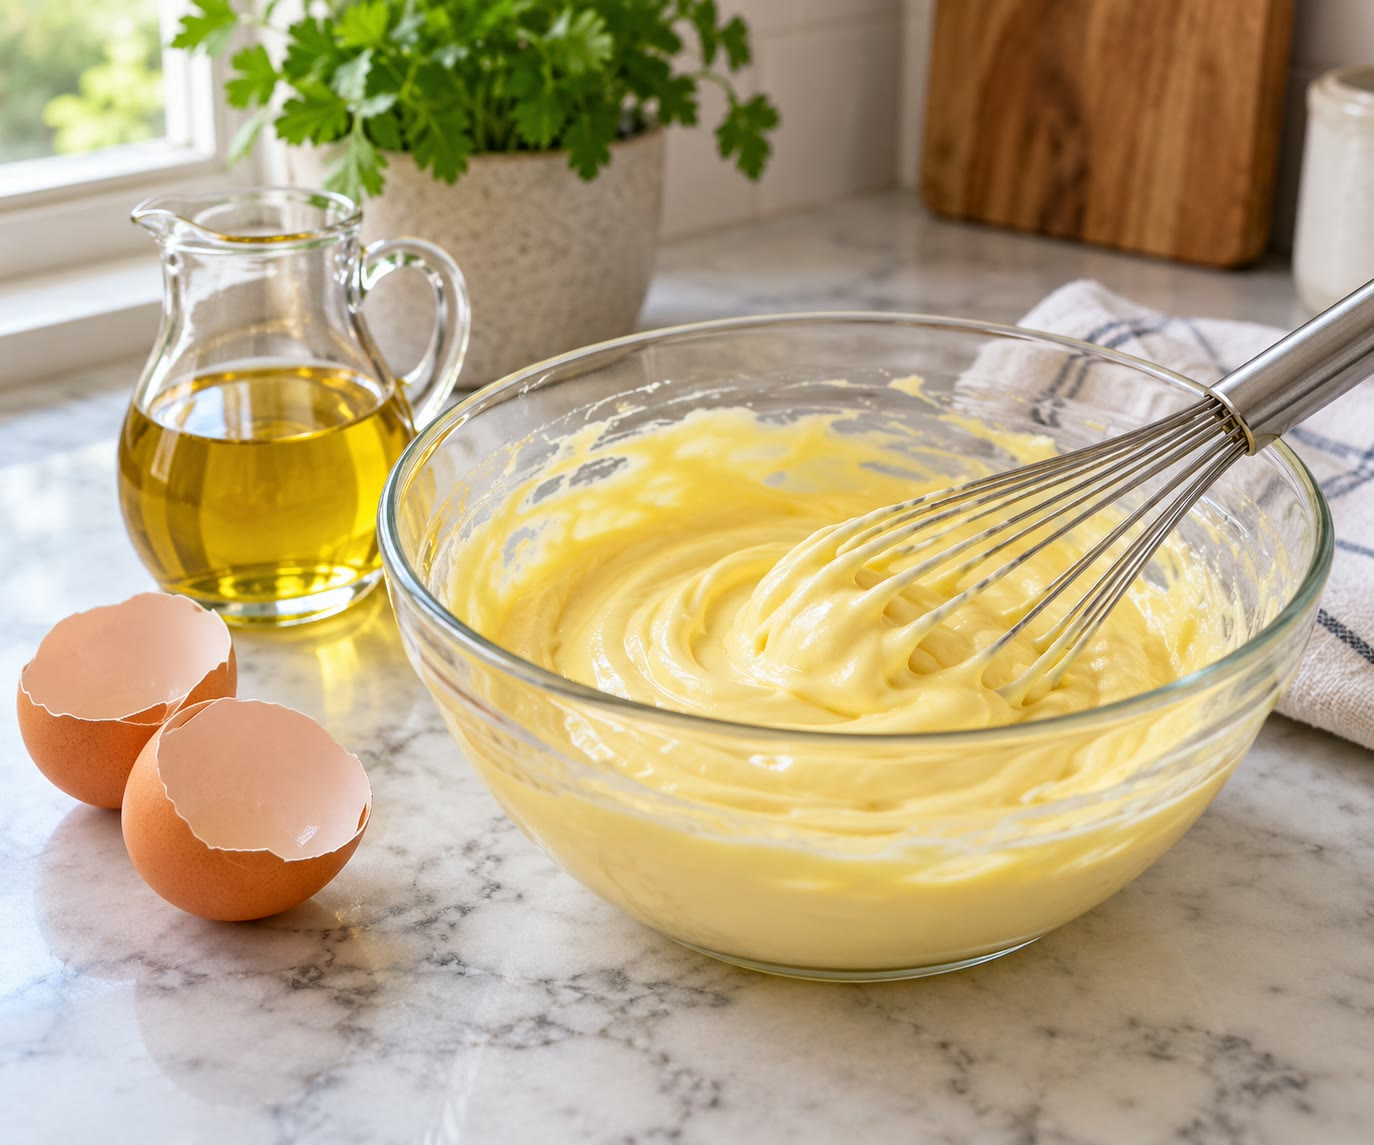
\includegraphics[width=0.6\linewidth]{images/book4/ai/b3-17-mayonnaise.jpg}

{\small Mayonaise wordt geklopt: een \omterm{def:b3:colloids:colloid}{emulsie} van oliedruppels in water,
gestabiliseerd door de oppervlakteactieve stoffen van eigeel.}
\end{omfigure}

\section{Grensvlakken en oppervlaktespanning}

Een molecuul in het inwendige van een vloeistof wordt in alle richtingen
even sterk aangetrokken; aan het oppervlak verliest het een deel van zijn
buren. Oppervlak scheppen kost energie.

\begin{definition}[Oppervlaktespanning]\label{def:b3:colloids:surface-tension}
De \emph{oppervlaktespanning}\index{oppervlaktespanning} $\gamma$ van een
vloeistof is de gibbsenergie die nodig is om een eenheid van oppervlakte
te scheppen bij constante temperatuur, druk en samenstelling: $\gamma = (\partial G/\partial A)_{T,p,n}$, in \unit{J.m^{-2}} $=$ \unit{N.m^{-1}}. Voor
een grensvlak tussen twee fasen is het de grensvlakspanning.
\end{definition}

Water, bijeengehouden door waterstofbruggen, heeft een hoge
\omterm{def:b3:colloids:surface-tension}{oppervlaktespanning}: \qty{72.0}{mN/m}
bij \qty{25}{\celsius}. Alkanen hebben ongeveer 20, kwik ongeveer 480.

\begin{proposition}[Druk van Laplace]\label{prop:b3:colloids:laplace}
De druk binnen een bolvormige druppel of bel met straal $r$ is groter dan
de druk buiten, met
\[
  \Delta p = \frac{2\gamma}{r} .
\]
\end{proposition}

\begin{proof}
Vergroot de straal in evenwicht met $\dd r$: de arbeid van het
drukverschil, $\Delta p\,4\pi r^2\dd r$, is gelijk aan de toename van de oppervlaktegibbsenergie, $\gamma\,8\pi r\,\dd r$.
\end{proof}

\begin{definition}[Contacthoek, bevochtiging]\label{def:b3:colloids:wetting}
De \emph{contacthoek}\index{contacthoek} $\theta$ van een druppel op een
vaste stof is de hoek, gemeten door de vloeistof heen, tussen het
oppervlak van de vaste stof en het vloeistofoppervlak, op de lijn waar
vaste stof, vloeistof en damp samenkomen. Een vloeistof
\emph{bevochtigt}\index{bevochtiging} de vaste stof als $\theta < 90^\circ$, en spreidt zich volledig uit als $\theta = 0$.
\end{definition}

\begin{theorem}[Vergelijking van Young]\label{thm:b3:colloids:young}
In evenwicht voldoen de drie grensvlakspanningen en de \omterm{def:b3:colloids:wetting}{contacthoek} aan
\[
  \gamma_{\mathrm{SV}} = \gamma_{\mathrm{SL}} + \gamma_{\mathrm{LV}}\cos\theta .
\]
Dit is de \emph{vergelijking van Young}\index{vergelijking van Young}.
\end{theorem}

\begin{proof}
Verschuif de contactlijn met $\dd x$ naar buiten (per lengte-eenheid van de
lijn): een grensvlak vaste stof-damp met oppervlakte $\dd x$ wordt vervangen door
een grensvlak vaste stof-vloeistof, en het grensvlak vloeistof-damp groeit met $\dd x\cos\theta$. De gibbsenergie
verandert met
$(\gamma_{\mathrm{SL}} - \gamma_{\mathrm{SV}} + \gamma_{\mathrm{LV}}\cos\theta)\dd x$, wat in evenwicht nul is.
\end{proof}

\begin{omfigure}
\begin{tikzpicture}[font=\small, >=Stealth]
  \fill[black!12] (-3.6,-0.5) rectangle (3.6,0);
  \draw[thick] (-3.6,0) -- (3.6,0);
  \node[anchor=north] at (2.6,-0.05) {vaste stof};
  \fill[omWater!60] (-2.0,0) arc[start angle=160, end angle=20, radius=2.13] -- cycle;
  \draw[thick, omDef] (-2.0,0) arc[start angle=160, end angle=20, radius=2.13];
  % circle centre 0.73 below the solid: a cap smaller than a hemisphere, contact angle 90 - 20 = 70 deg;
  % at the right contact point the liquid surface leaves at 110 deg (up and to the left)
  \draw[->, thick, omThm] (2.0,0) -- ++(110:1.3) node[anchor=south] {$\gamma_{\mathrm{LV}}$};
  \draw[->, thick] (2.0,0) -- (3.3,0) node[anchor=south] {$\gamma_{\mathrm{SV}}$};
  \draw[->, thick] (2.0,0) -- (0.7,0) node[anchor=north, yshift=-1pt] {$\gamma_{\mathrm{SL}}$};
  \draw (1.45,0) arc[start angle=180, end angle=110, radius=0.55];
  \node at (1.33,0.42) {$\theta$};
  \node at (0,0.6) {vloeistof};
  \node at (-2.8,1.4) {damp};
\end{tikzpicture}

{\small Een liggende druppel en de drie spanningen die aan zijn contactlijn
trekken: het evenwicht van hun componenten langs de vaste stof geeft de
\omterm{thm:b3:colloids:young}{vergelijking van Young}; hier is $\theta
\approx 70^\circ$, een gedeeltelijk bevochtigende vloeistof.}
\end{omfigure}

\begin{theorem}[Vergelijking van Kelvin]\label{thm:b3:colloids:kelvin}
De dampdruk van een bolvormige druppel met straal $r$ is groter dan die
van de vlakke vloeistof, $p^*$:
\[
  \ln\frac{p}{p^*} = \frac{2\gamma V_{\mathrm m}}{rRT},
\]
met $V_{\mathrm m}$ het molair volume van de vloeistof. Dit is de
\emph{vergelijking van Kelvin}\index{vergelijking van Kelvin}.
\end{theorem}

\begin{proof}
De vloeistof in de druppel staat onder de extra druk $2\gamma/r$, die haar
chemische potentiaal verhoogt met $V_{\mathrm m}\,2\gamma/r$ (met $(\partial\mu/\partial p)_T = V_{\mathrm m}$, de vloeistof onsamendrukbaar).
De damp die ermee in evenwicht is, moet haar chemische potentiaal met
hetzelfde bedrag zien stijgen: $RT\ln(p/p^*) = 2\gamma V_{\mathrm m}/r$.
\end{proof}

Voor een waterdruppel met straal \qty{10}{nm} bij \qty{25}{\celsius} is $2\gamma V_{\mathrm m}/rRT = 0.105$: zijn
dampdruk ligt 11\,\% boven die van vlak water. Kleine druppels verdampen
terwijl grote groeien, en wolken hebben kernen nodig om te ontstaan;
hetzelfde geldt voor de oplosbaarheid van kleine kristallen.

\begin{definition}[Ostwaldrijping]\label{def:b3:colloids:ripening}
\emph{Ostwaldrijping}\index{ostwaldrijping} is de groei van de grotere
deeltjes of druppels van een dispersie ten koste van de kleinere,
gedreven door de hogere oplosbaarheid of dampdruk van kleine deeltjes.
\end{definition}

\section{Oppervlakteactieve stoffen en micellen}

\begin{definition}[Oppervlakteactieve stof]\label{def:b3:colloids:surfactant}
Een \emph{oppervlakteactieve stof}\index{oppervlakteactieve stof}
(surfactant) is een amfifiel molecuul dat aan grensvlakken adsorbeert en
hun spanning verlaagt. Het is een
\emph{anionische oppervlakteactieve stof}\index{anionische oppervlakteactieve stof}
als zijn kop een anion is (natriumdodecylsulfaat, zepen), een
\emph{kationische oppervlakteactieve stof}\index{kationische oppervlakteactieve stof}
als hij een kation is (quaternaire ammoniumzouten), een
\emph{niet-ionische oppervlakteactieve
stof}\index{niet-ionische oppervlakteactieve stof} als de kop een neutrale
polaire groep is (een keten van ethyleenoxide-eenheden).
\end{definition}

\begin{definition}[Oppervlakte-excesconcentratie]\label{def:b3:colloids:surface-excess}
De \emph{oppervlakte-excesconcentratie}\index{oppervlakte-excesconcentratie} $\Gamma$ van een
opgeloste stof is de hoeveelheid opgeloste stof aan het grensvlak per
oppervlakte-eenheid, bovenop wat hetzelfde volume zou bevatten als de
concentratie van het inwendige tot aan het grensvlak gold.
\end{definition}

\begin{theorem}[Adsorptie-isotherm van Gibbs]\label{thm:b3:colloids:gibbs-adsorption}
Voor een verdunde oplossing van een niet-ionische opgeloste stof met
concentratie $c$ is
\[
  \Gamma = -\frac{1}{RT}\frac{\dd\gamma}{\dd\ln c};
\]
voor een ionische \omterm{def:b3:colloids:surfactant}{oppervlakteactieve stof} van het type 1:1 zonder
toegevoegd zout wordt $RT$ vervangen door $2RT$. Dit is
de \emph{adsorptie-isotherm van Gibbs}\index{adsorptie-isotherm van Gibbs}.
\end{theorem}

\begin{proof}
Voor het grensvlak is de tegenhanger van de betrekking van Gibbs-Duhem bij constante $T$ en
$p$ de betrekking $\dd\gamma = -\sum_i\Gamma_i\,\dd\mu_i$ (de oppervlaktegibbsenergie $\gamma A$ speelt de rol van $G$;
aangenomen). Kiest men het scheidingsvlak zo dat het oplosmiddel geen
exces heeft, dan is
$\dd\gamma = -\Gamma\,\dd\mu$, en in een verdunde oplossing is $\dd\mu = RT\,\dd\ln c$. Bij een ionische \omterm{def:b3:colloids:surfactant}{oppervlakteactieve stof}
worden het kation en het anion allebei met hetzelfde exces geadsorbeerd en
wordt $\dd\mu$
$2RT\,\dd\ln c$.
\end{proof}

Een \omterm{def:b3:colloids:surfactant}{oppervlakteactieve stof} waarvan de \omterm{def:b3:colloids:surface-tension}{oppervlaktespanning} lineair daalt
met $\ln c$, heeft een constant
oppervlakte-exces: het grensvlak is verzadigd, en $1/(\Gamma N_A)$ is de oppervlakte die
één geadsorbeerd molecuul inneemt.

\begin{method}[Oppervlakte per molecuul uit een helling $\gamma$--$\ln c$]\label{met:b3:colloids:surface-excess}
\begin{enumerate}
  \item Meet $\gamma$ als functie van $c$ onder de CMC; zet $\gamma$ uit tegen $\ln c$.
  \item Neem de helling van het lineaire deel net onder de CMC; $\Gamma = -\text{helling}/(nRT)$, $n
        = 1$ voor een \omterm{def:b3:colloids:surfactant}{niet-ionische oppervlakteactieve stof}, 2 voor een
        ionische van het type 1:1 zonder zout.
  \item Oppervlakte per molecuul $= 1/(\Gamma N_A)$; typische waarden zijn 0.3 tot \qty{0.6}{nm^2}.
\end{enumerate}
\end{method}

\begin{definition}[Micel, kritische micelconcentratie, aggregatiegetal]\label{def:b3:colloids:micelle}
Een \emph{micel}\index{micel} is een aggregaat van moleculen van een
\omterm{def:b3:colloids:surfactant}{oppervlakteactieve stof} in oplossing, waarvan de hydrofobe staarten een
vloeistofachtige kern vormen die door de koppen van het water
afgeschermd wordt. De \emph{kritische micelconcentratie}\index{kritische micelconcentratie}
(CMC) is de concentratie waarboven micellen ontstaan; hun gemiddelde
aantal moleculen is het \emph{aggregatiegetal}\index{aggregatiegetal}.
\end{definition}

\begin{proposition}[Knikken bij de CMC]\label{prop:b3:colloids:cmc-break}
Boven de CMC blijven de concentratie van de vrije \omterm{def:b3:colloids:surfactant}{oppervlakteactieve
stof}, en daarmee de \omterm{def:b3:colloids:surface-tension}{oppervlaktespanning} en de osmotische druk, vrijwel
constant; eigenschappen die van de vrije moleculen afhangen, veranderen
van helling bij de CMC.
\end{proposition}

\begin{proof}[Gedeeltelijk bewijs]
Beschouw de \omterm{def:b3:colloids:micelle}{micellen} als een afzonderlijke fase: toegevoegde
\omterm{def:b3:colloids:surfactant}{oppervlakteactieve stof} gaat naar de \omterm{def:b3:colloids:micelle}{micellen} zodra de chemische
potentiaal van de vrije moleculen die van een molecuul in een \omterm{def:b3:colloids:micelle}{micel}
bereikt, en deze chemische potentiaal, en dus de vrije concentratie,
blijft daarna vast. De \omterm{def:b3:colloids:surface-tension}{oppervlaktespanning}, die via de isotherm van Gibbs
door de vrije moleculen bepaald wordt, daalt niet meer; de geleidbaarheid
blijft stijgen, maar trager, omdat \omterm{def:b3:colloids:micelle}{micellen} per molecuul minder lading
dragen dan vrije ionen (een deel van hun tegenionen is gebonden). Het
model is een limiet, want \omterm{def:b3:colloids:micelle}{micellen} van eindige grootte ontstaan over een
smal concentratiegebied (aangenomen).
\end{proof}

\begin{method}[De CMC uit een knik]\label{met:b3:colloids:cmc}
\begin{enumerate}
  \item Meet de \omterm{def:b3:colloids:surface-tension}{oppervlaktespanning} (of, voor een ionische
        \omterm{def:b3:colloids:surfactant}{oppervlakteactieve stof}, de geleidbaarheid) over een
        concentratiegebied rond de verwachte CMC.
  \item Pas rechten aan de twee takken aan ($\gamma$ tegen $\log c$, of $\kappa$ tegen $c$).
  \item Hun snijpunt is de CMC.
\end{enumerate}
\end{method}

\begin{omfigure}
\begin{tikzpicture}
\begin{axis}[name=gm, width=0.47\linewidth, height=5.2cm, xmin=-5, xmax=-1.5, ymin=30, ymax=76,
  axis lines=left, xlabel={$\log(c/\unit{mol.L^{-1}})$}, ylabel={$\gamma$ / \unit{mN.m^{-1}}},
  tick label style={font=\small}, label style={font=\small}]
\addplot[omDef, very thick] table[x=logc, y=gamma_mN] {figdata/out/bachelor-3-surfactant-cmc-gamma.dat};
\draw[black!40, dashed] (axis cs:-2.086,30) -- (axis cs:-2.086,70);
\node[font=\scriptsize, anchor=south west] at (axis cs:-2.05,45) {CMC};
\end{axis}
\begin{axis}[at={(gm.east)}, anchor=west, xshift=1.4cm, width=0.47\linewidth, height=5.2cm,
  xmin=0, xmax=20, ymin=0, ymax=1.0, axis lines=left, xlabel={$c$ / mM},
  ylabel={$\kappa$ / \unit{mS.cm^{-1}}}, tick label style={font=\small}, label style={font=\small}]
\addplot[omThm, very thick] table[x=c_mM, y=kappa] {figdata/out/bachelor-3-surfactant-cmc-kappa.dat};
\draw[black!40, dashed] (axis cs:8.2,0) -- (axis cs:8.2,0.9);
\node[font=\scriptsize, anchor=south west] at (axis cs:8.4,0.15) {CMC};
\end{axis}
\end{tikzpicture}

{\small Een modelionische \omterm{def:b3:colloids:surfactant}{oppervlakteactieve stof} met de CMC van
natriumdodecylsulfaat,
\qty{8.2}{mM} bij \qty{25}{\celsius}. Links: de \omterm{def:b3:colloids:surface-tension}{oppervlaktespanning} daalt met $\log c$, lineair net onder
de CMC (een verzadigd grensvlak, ongeveer \qty{0.6}{nm^2} per molecuul), en blijft
daarna constant. Rechts: de geleidbaarheid stijgt boven de CMC minder
steil.}
\end{omfigure}

\begin{definition}[Pakkingsparameter]\label{def:b3:colloids:packing}
De \emph{pakkingsparameter}\index{pakkingsparameter} van een
\omterm{def:b3:colloids:surfactant}{oppervlakteactieve stof} is $P =
v/(a_0l)$, waarin $v$ het volume van zijn hydrofobe staart is, $l$ de lengte van de
gestrekte staart en $a_0$ de optimale oppervlakte per kopgroep aan het
oppervlak van het aggregaat.
\end{definition}

\begin{proposition}[Vorm van de aggregaten]\label{prop:b3:colloids:packing}
Bolvormige \omterm{def:b3:colloids:micelle}{micellen} vereisen $P \le \frac13$, cilindrische \omterm{def:b3:colloids:micelle}{micellen} $\frac13 < P \le \frac12$, vlakke bilagen
(vesikels, membranen) $\frac12 < P \le 1$; $P > 1$ geeft omgekeerde structuren.
\end{proposition}

\begin{proof}
In een bol met straal $R \le l$ uit $N$ moleculen is $Nv = \frac43\pi R^3$ en $Na_0 = 4\pi R^2$, dus
$v/a_0 = R/3 \le l/3$: $P \le \frac13$. Voor een cilinder met straal $R$ en lengte $L$ is $Nv = \pi R^2L$ en
$Na_0 = 2\pi RL$: $v/a_0 = R/2 \le l/2$. Voor een bilaag met dikte $2l$ en oppervlakte $A$ is $Nv = 2lA$ en
$Na_0 = 2A$: $v/a_0 = l$.
\end{proof}

\begin{omfigure}
\begin{tikzpicture}[font=\scriptsize]
  % a sphere-forming cone
  \draw[omDef, thick, fill=omDef!15] (0,0) -- (-0.45,1.2) arc[start angle=180, end angle=0, radius=0.45] -- cycle;
  \node at (0,-0.3) {$P < \frac13$: kegel};
  % micelle
  \begin{scope}[xshift=2.2cm, yshift=0.6cm]
    \foreach \a in {0,30,...,330}{\draw[black!60] (\a:0.2) -- (\a:0.62); \fill[omDef] (\a:0.7) circle (0.09);}
    \node at (0,-1.05) {bolvormige micel};
  \end{scope}
  % truncated cone
  \begin{scope}[xshift=4.7cm]
    \draw[omDef, thick, fill=omDef!15] (-0.18,0) -- (-0.4,1.2) -- (0.4,1.2) -- (0.18,0) -- cycle;
    \node at (0,-0.3) {$\frac13 < P < \frac12$};
  \end{scope}
  \begin{scope}[xshift=6.9cm, yshift=0.6cm]
    \fill[omDef!10] (-0.9,-0.55) rectangle (0.9,0.55);
    \foreach \x in {-0.8,-0.5,...,0.8}{\fill[omDef] (\x,0.62) circle (0.08); \fill[omDef] (\x,-0.62) circle (0.08);}
    \node at (0,-1.05) {cilinder (zijaanzicht)};
  \end{scope}
  % cylinder shape
  \begin{scope}[xshift=9.4cm]
    \draw[omDef, thick, fill=omDef!15] (-0.3,0) rectangle (0.3,1.2);
    \node at (0,-0.3) {$P \approx 1$: cilinder};
  \end{scope}
  \begin{scope}[xshift=11.4cm, yshift=0.6cm]
    \foreach \x in {-0.8,-0.6,...,0.8}{
      \draw[black!60] (\x,0.5) -- (\x,0.05) (\x,-0.5) -- (\x,-0.05);
      \fill[omDef] (\x,0.58) circle (0.08); \fill[omDef] (\x,-0.58) circle (0.08);}
    \node at (0,-1.05) {bilaag};
  \end{scope}
\end{tikzpicture}

{\small Vorm van het molecuul en vorm van het aggregaat. Een
\omterm{def:b3:colloids:surfactant}{oppervlakteactieve stof} met een grote kop en één staart (een kegel)
pakt zich in bolvormige \omterm{def:b3:colloids:micelle}{micellen}; met een kleinere kop in cilinders; een
molecuul dat aan de staart even breed is als aan de kop, zoals een lipide
met twee ketens, in vlakke bilagen, de wanden van vesikels en
celmembranen.}
\end{omfigure}

Bij het reinigen werken deze effecten samen: de \omterm{def:b3:colloids:surfactant}{oppervlakteactieve stof}
verlaagt de grensvlakspanning tussen water en een vettig vuil tot het
vuil zich tot druppels oprolt, die \omterm{def:b3:colloids:micelle}{micellen} daarna in hun kern oplossen.

\section{Colloïden}

\begin{definition}[Colloïd]\label{def:b3:colloids:colloid}
Een \emph{colloïd}\index{colloid@colloïd} is een dispersie van deeltjes,
druppels of bellen van ruwweg
\qty{1}{nm} tot \qty{1}{\micro m} groot (de \emph{gedispergeerde fase}\index{gedispergeerde fase}),
in een continu \emph{dispersiemedium}\index{dispersiemedium}. Een
\emph{sol}\index{sol} is een dispersie van vaste deeltjes in een
vloeistof, een \emph{emulsie}\index{emulsie} een dispersie van
vloeistofdruppels in een andere vloeistof, een
\emph{schuim}\index{schuim} een dispersie van gasbellen in een vloeistof
of een vaste stof, een \emph{gel}\index{gel}
een netwerk van deeltjes of polymeren dat de hele vloeistof doortrekt en
haar vastestofachtig maakt, een \emph{aerosol}\index{aerosol} een
dispersie van druppels of deeltjes in een gas.
\end{definition}

Colloïdale deeltjes zijn klein genoeg om door de brownse beweging (de
willekeurige stoten van oplosmiddelmoleculen, uit de natuurkunde) in
suspensie te blijven en groot genoeg om licht te verstrooien.

\begin{definition}[Tyndalleffect]\label{def:b3:colloids:tyndall}
Het \emph{tyndalleffect}\index{tyndalleffect} is de verstrooiing van licht
door de deeltjes van een \omterm{def:b3:colloids:colloid}{colloïd}, waardoor een lichtbundel die het
\omterm{def:b3:colloids:colloid}{colloïd} doorkruist van opzij zichtbaar wordt, terwijl een echte oplossing
onzichtbaar blijft.
\end{definition}

\begin{omfigure}

\includegraphics[width=0.55\linewidth]{images/book4/tyndall-sky.jpg}

{\small Zonnestralen door een opening in de wolken: ze zijn zichtbaar
omdat het \omterm{def:b3:colloids:colloid}{aerosol} van de lucht, druppeltjes en stof, een deel van het
licht zijwaarts verstrooit, het \omterm{def:b3:colloids:tyndall}{tyndalleffect} op de schaal van de
hemel.}
\end{omfigure}

\section{Stabiliteit van colloïden}

Twee colloïdale deeltjes trekken elkaar op korte afstand altijd aan door
vanderwaalskrachten. In water dragen de meeste deeltjes bovendien een
lading (geïoniseerde oppervlaktegroepen, geadsorbeerde ionen), omringd
door een \omterm{def:b3:electrode-kinetics:double-layer}{diffuse laag} van tegenionen, de dubbellaag van
\cref{ch:b3:electrode-kinetics}. Wanneer twee deeltjes elkaar naderen,
overlappen hun diffuse lagen en stoten ze elkaar af.

\begin{definition}[Zetapotentiaal]\label{def:b3:colloids:zeta}
De \emph{zetapotentiaal}\index{zetapotentiaal} $\zeta$ van een deeltje is
de elektrische potentiaal op zijn afschuifvlak, de grens binnen de
dubbellaag tussen de vloeistof die met het deeltje meebeweegt en de
vloeistof die dat niet doet; hij wordt gemeten uit de snelheid van de
deeltjes in een elektrisch veld (elektroforese).
\end{definition}

\begin{omfigure}
\begin{tikzpicture}[font=\scriptsize]
  \fill[black!20] (0,0) circle (1.2);
  \foreach \a in {0,30,...,330}{\node at (\a:1.05) {$-$};}
  \draw[omDef, dashed] (0,0) circle (1.55);
  \foreach \a in {15,45,...,345}{\draw[omDef, fill=omDef!15] (\a:1.38) circle (0.11); \node at (\a:1.38) {\tiny$+$};}
  \draw[omThm, thick, densely dotted] (0,0) circle (1.85);
  \foreach \a/\r/\s in {10/2.2/+, 50/2.5/+, 95/2.3/-, 130/2.7/+, 175/2.2/+, 215/2.6/-, 250/2.3/+, 290/2.8/+, 345/2.6/+}{
    \draw[black!60, fill=white] (\a:\r) circle (0.11); \node at (\a:\r) {\tiny$\s$};}
  \draw[->, black!60] (2.6,1.6) node[anchor=west] {sternlaag} -- (40:1.6);
  \draw[->, omThm] (2.6,-1.4) node[anchor=west] {afschuifvlak: $\zeta$} -- (-30:1.87);
  \node at (0,0) {deeltje};
  \node[anchor=west] at (2.9,0.2) {diffuse laag};
\end{tikzpicture}

{\small Een negatief geladen deeltje met zijn dubbellaag: een compacte
sternlaag van tegenionen, het afschuifvlak net daarbuiten, waar de
\omterm{def:b3:colloids:zeta}{zetapotentiaal} gedefinieerd is, en de \omterm{def:b3:electrode-kinetics:double-layer}{diffuse laag}, waarin de tegenionen
over enkele \omterm{def:b3:electrode-kinetics:double-layer}{debyelengten} talrijker zijn dan de co-ionen.}
\end{omfigure}

\begin{theorem}[DLVO-theorie]\label{thm:b3:colloids:dlvo}
Voor twee bollen met straal $a$, gescheiden door een spleet $h \ll a$, met
potentiaal van de \omterm{def:b3:electrode-kinetics:double-layer}{diffuse laag}
$\psi$ en hamakerconstante $A$, is de interactie-energie bij lage
potentialen
\[
  V(h) = 2\pi\varepsilon_r\varepsilon_0a\psi^2\ln\bigl(1 + \eu^{-\kappa h}\bigr) - \frac{Aa}{12h} .
\]
De eerste term, de afstoting van de dubbellagen, neemt af over de \omterm{def:b3:electrode-kinetics:double-layer}{debyelengte} $\kappa^{-1}$;
de tweede, de vanderwaalsaantrekking, hangt niet van het zout af. Hun som
heeft een energiebarrière op enkele \omterm{def:b3:electrode-kinetics:double-layer}{debyelengten} wanneer de
zoutconcentratie laag is, en geen enkele boven een kritische
concentratie.
\end{theorem}

\begin{proof}[Gedeeltelijk bewijs]
Beide vormen worden aangenomen (de afstoting uit de overlap van twee lagen
van Gouy-Chapman in de benadering van Derjaguin, de aantrekking uit de
sommatie van londoninteracties over de twee lichamen). Een hogere
ionsterkte verhoogt $\kappa$
(\cref{prop:b3:electrode-kinetics:debye-length}): de afstoting sterft dan
uit bij kleinere $h$, waar de aantrekking, die groeit als $1/h$, sterker is; het maximum
van $V$ neemt af en verdwijnt ten slotte.
\end{proof}

\begin{omfigure}
\begin{tikzpicture}
\begin{axis}[width=0.72\linewidth, height=5.6cm, xmin=0, xmax=30, ymin=-40, ymax=45,
  axis lines=left, xlabel={spleet $h$ / nm}, ylabel={$V/kT$},
  tick label style={font=\small}, label style={font=\small},
  legend style={font=\scriptsize, draw=none, at={(0.98,0.98)}, anchor=north east}, legend cell align=left]
\addplot[omDef, thick] table[x=h_nm, y=I1] {figdata/out/bachelor-3-dlvo.dat};
\addplot[black!60, thick] table[x=h_nm, y=I10] {figdata/out/bachelor-3-dlvo.dat};
\addplot[omThm, thick] table[x=h_nm, y=I50] {figdata/out/bachelor-3-dlvo.dat};
\addplot[black, thick, dashed] table[x=h_nm, y=I200] {figdata/out/bachelor-3-dlvo.dat};
\draw[black!30] (axis cs:0,0) -- (axis cs:30,0);
\legend{\qty{1}{mM}, \qty{10}{mM}, \qty{50}{mM}, \qty{200}{mM}}
\end{axis}
\end{tikzpicture}

{\small DLVO-interactie van twee deeltjes met straal \qty{100}{nm} (model:
potentiaal van de \omterm{def:b3:electrode-kinetics:double-layer}{diffuse laag}
\qty{-30}{mV}, hamakerconstante \qty{2e-20}{J}) in water met een zout van het type 1:1. Bij \qty{1}{mM}
houdt een barrière van ongeveer $40\,kT$ de deeltjes uit elkaar; bij \qty{10}{mM} is ze gehalveerd;
rond \qty{50}{mM} verdwijnt ze en blijft elke botsing kleven.}
\end{omfigure}

\begin{definition}[Coagulatie en stabilisatie]\label{def:b3:colloids:stability}
\emph{Coagulatie}\index{coagulatie} is de aggregatie van colloïdale
deeltjes door het verlies van hun elektrostatische afstoting;
\emph{flocculatie}\index{flocculatie}
is aggregatie tot losse vlokken, vaak overbrugd door geadsorbeerde
polymeren. De
\emph{kritische coagulatieconcentratie}\index{kritische coagulatieconcentratie}
(CCC) van een elektrolyt is de concentratie waarboven een \omterm{def:b3:colloids:colloid}{colloïd} snel
coaguleert. \emph{Sterische stabilisatie}\index{sterische stabilisatie}
houdt deeltjes uit elkaar met geadsorbeerde of geënte polymeerketens,
waarvan de overlap entropie zou kosten.
\end{definition}

\begin{proposition}[Regel van Schulze-Hardy]\label{prop:b3:colloids:schulze-hardy}
Voor een sterk geladen \omterm{def:b3:colloids:colloid}{colloïd} varieert de \omterm{def:b3:colloids:stability}{kritische
coagulatieconcentratie} van een elektrolyt als de omgekeerde zesde macht
van de lading $z$ van zijn
tegenionen: $\text{CCC} \propto z^{-6}$, in de verhoudingen $1 : \frac{1}{64} : \frac{1}{729}$ voor $z = 1, 2, 3$.
\end{proposition}

\begin{proof}[Gedeeltelijk bewijs]
Beschouw twee vlakke platen. Bij een hoge oppervlaktepotentiaal nadert de
afstoting van de dubbellagen per oppervlakte-eenheid $V_R = (64nkT/\kappa)\eu^{-\kappa h}$, met $n$ de deeltjesdichtheid van de $z{:}z$-elektrolyt,
onafhankelijk van de potentiaal (aangenomen); de aantrekking is $V_A =
-A/(12\pi h^2)$. Bij de CCC verdwijnt de barrière net: $V = 0$ en $\dd V/\dd h = 0$ bij dezelfde
spleet. Omdat $\dd V_R/\dd h = -\kappa V_R$ en $\dd V_A/\dd h = -2V_A/h$, geven de twee voorwaarden
$\kappa V_R = 2V_R/h$, dus $\kappa h = 2$, en dan $64nkT\eu^{-2}/\kappa = A\kappa^2/(48\pi)$, d.w.z.\ $n \propto \kappa^3$. Met
$\kappa^2 = 2nz^2e^2/(\varepsilon kT)$ is $\kappa^3 \propto (nz^2)^{3/2}$ en $n \propto n^{3/2}z^3$: dus $n \propto z^{-6}$.
\end{proof}

\begin{omfigure}
\begin{tikzpicture}[font=\small, >=Stealth]
  \foreach \x/\lab/\v in {0/\ce{Na+}/1, 2.6/\ce{Ca^{2+}}/{1/64}, 5.2/\ce{Al^{3+}}/{1/729}}{
    \node at (\x,0) {\lab};
    \node[font=\scriptsize] at (\x,-0.45) {CCC $\times\,\v$};}
  \draw[->, thick, omDef] (-0.8,-0.95) -- (6.0,-0.95) node[midway, below, font=\scriptsize] {kleinere dosis om een negatief colloïd te coaguleren};
\end{tikzpicture}

{\small De regel van Schulze-Hardy voor een negatief geladen \omterm{def:b3:colloids:colloid}{colloïd}: de
\omterm{def:b3:colloids:stability}{kritische coagulatieconcentratie} daalt met de zesde macht van de lading
van het tegenion.}
\end{omfigure}

De regel verklaart waarom aluminiumzouten zo doeltreffend water klaren,
en waarom rivieren hun lading klei laten vallen waar ze het zoute water
van de zee ontmoeten.

\begin{method}[Een coagulantdosis kiezen]\label{met:b3:colloids:coagulant-dose}
\begin{enumerate}
  \item Meet de CCC van een referentie-elektrolyt voor de suspensie
        (bekerproeven met toenemende doses, waarbij je het bezinken
        volgt).
  \item Herschaal haar naar het tegenion van het coagulant met de regel
        van Schulze-Hardy.
  \item Reken met de formule om naar een massa zout per kubieke meter;
        voeg genoeg toe voor de hydrolyse en de alkaliniteit die die
        verbruikt.
  \item Vermijd overdosering: sterk geladen tegenionen kunnen het teken
        van de lading van de deeltjes omkeren en ze opnieuw
        stabiliseren.
\end{enumerate}
\end{method}

\section{Colloïden aan het werk}

\begin{definition}[Hydrofiel-lipofiele balans]\label{def:b3:colloids:hlb}
De \emph{hydrofiel-lipofiele balans}\index{hydrofiel-lipofiele balans}
(HLB) van een \omterm{def:b3:colloids:surfactant}{niet-ionische oppervlakteactieve stof} is, op de schaal van
Griffin, $20$ maal de
massafractie van haar hydrofiele deel: lage waarden (3 tot 6) passen bij
water-in-olie-emulsies, hoge waarden (8 tot 18) bij olie-in-water-emulsies
en detergenten.
\end{definition}

\omterm{def:b3:colloids:colloid}{Emulsies} zijn thermodynamisch instabiel, omdat elke druppel
grensvlakenergie draagt; emulgatoren maken ze kinetisch stabiel door die
energie te verlagen en door rond elke druppel een afstotende laag toe te
voegen, geladen of sterisch. Mayonaise is een olie-in-water-emulsie met
zoveel olie (ongeveer vier vijfde van het volume) dat de druppels tegen
elkaar gedrukt worden, wat haar tot een zachte vaste stof maakt. \omterm{def:b3:colloids:colloid}{Schuimen}
worden gestabiliseerd door oppervlakteactieve stoffen die het uitzakken
van de vloeistoffilms tussen de bellen vertragen; antischuimmiddelen,
vaak siliconenoliën, spreiden zich over die films uit en breken ze. In
drinkwaterbedrijven coaguleren aluminium- of ijzer(III)zouten de klei- en
organische \omterm{def:b3:colloids:colloid}{colloïden} die rivierwater troebel maken; het hydroxide dat ze
vormen, sleept de vlokken bij het bezinken mee naar beneden.
Metaalnanodeeltjes worden gedispergeerd gehouden door geadsorbeerde
citraationen (elektrostatisch) of door via thiolen gebonden
polymeerketens (sterisch).

\begin{inthelab}[De ring van Du Noüy]
Een platinaring, in de vlam gereinigd, hangt aan een balans en wordt
horizontaal in de vloeistof gedompeld en daarna langzaam opgetild. De
kracht die nodig is om hem door het oppervlak te trekken, gaat door een
maximum; gedeeld door tweemaal de omtrek van de ring en gecorrigeerd voor
de vorm van de opgetilde meniscus geeft ze de \omterm{def:b3:colloids:surface-tension}{oppervlaktespanning}. De
meting van een reeks oplossingen van een \omterm{def:b3:colloids:surfactant}{oppervlakteactieve stof} begint
bij de meest verdunde, en de ring wordt tussen de monsters gespoeld.
\end{inthelab}

\begin{safety}{\ghs[0.8cm]{GHS02}\ghs[0.8cm]{GHS05}\ghs[0.8cm]{GHS07}}
% ledger: ghs4:SDS, ghs4:Al2SO43
Natriumdodecylsulfaatpoeder: ontvlambare vaste stof, schadelijk bij
inslikken, veroorzaakt ernstig oogletsel, irriteert de luchtwegen; afwegen
zonder stof op te werpen, met oogbescherming. Aluminiumsulfaat (\ghs[0.6cm]{GHS05}):
veroorzaakt ernstig oogletsel.
\end{safety}

\begin{history}[Tyndall en de ultramicroscoop]
John Tyndall toonde in 1869 aan dat een lichtbundel zichtbaar wordt in
lucht vol fijne deeltjes en onzichtbaar in lucht die ervan ontdaan is, en
dat het verstrooide licht blauwachtig en gepolariseerd is. Richard
Zsigmondy, die de rode kleur van goudsolen bestudeerde, bouwde in 1903 met
Henry Siedentopf de ultramicroscoop, die het \omterm{def:b3:colloids:colloid}{colloïd} van opzij belicht en
elk deeltje toont als een punt van verstrooid licht op een donkere
achtergrond, te klein om opgelost te worden maar telbaar. Hij ontving de
Nobelprijs voor de Scheikunde van 1925 voor zijn werk over \omterm{def:b3:colloids:colloid}{colloïden}.
\end{history}

\section{Oefeningen}

\begin{exercise}[$\star$]\label{exo:b3:colloids:1}
% ledger: st:H2O.25C
Bereken de druk binnen een luchtbel met diameter \qty{1.0}{\micro m} in water bij
\qty{25}{\celsius} (buiten: \qty{1.0}{bar}).
\end{exercise}

\begin{exercise}[$\star$]\label{exo:b3:colloids:2}
% ledger: st:H2O.25C
Bereken de dampdruk van een waterdruppel met straal \qty{10}{nm} ten
opzichte van vlak water bij \qty{25}{\celsius} ($V_{\mathrm m} = \qty{18.07}{cm^3/mol}$).
\end{exercise}

\begin{exercise}[$\star$]\label{exo:b3:colloids:3}
Een vloeistof met $\gamma_{\mathrm{LV}} = \qty{72}{mN/m}$ op een vaste stof met $\gamma_{\mathrm{SV}} = \qty{40}{mN/m}$ en $\gamma_{\mathrm{SL}} =
\qty{20}{mN/m}$ (gegevens van de oefening): bereken de \omterm{def:b3:colloids:wetting}{contacthoek}.
\omterm{def:b3:colloids:wetting}{Bevochtigt} ze de vaste stof?
\end{exercise}

\begin{exercise}[$\star$]\label{exo:b3:colloids:4}
% ledger: eps:H2O.25C
Bereken de \omterm{def:b3:electrode-kinetics:double-layer}{debyelengte} in water bij \qty{25}{\celsius} voor \qty{0.010}{mol/L} NaCl en voor
\ce{MgSO4}.
\end{exercise}

\begin{exercise}[$\star\star$]\label{exo:b3:colloids:5}
Net onder haar CMC daalt de \omterm{def:b3:colloids:surface-tension}{oppervlaktespanning} van een ionische
\omterm{def:b3:colloids:surfactant}{oppervlakteactieve stof} (1:1, zonder zout) met \qty{12.6}{mN/m} per eenheid van $\ln c$ bij \qty{25}{\celsius}. Bereken het
oppervlakte-exces en de oppervlakte per molecuul.
\end{exercise}

\begin{exercise}[$\star\star$]\label{exo:b3:colloids:6}
\omterm{def:b3:colloids:surface-tension}{Oppervlaktespanningen} van een \omterm{def:b3:colloids:surfactant}{niet-ionische oppervlakteactieve stof}: 52.0,
45.5, 39.1, 33.4, 33.3 en
\qty{33.4}{mN/m} bij $\log c = -5.0$, $-4.5$, $-4.0$, $-3.5$, $-3.0$ en $-2.5$ (gegevens van de oefening).
Schat de CMC.
\end{exercise}

\begin{exercise}[$\star\star$]\label{exo:b3:colloids:7}
Neem voor natriumdodecylsulfaat $v = \qty{0.350}{nm^3}$, $l = \qty{1.67}{nm}$ en $a_0 = \qty{0.60}{nm^2}$; voor een
lipide met twee zulke ketens $2v$, dezelfde $l$ en $a_0 = \qty{0.65}{nm^2}$ (gegevens van de
oefening). Voorspel de vorm van hun aggregaten.
\end{exercise}

\begin{exercise}[$\star\star$]\label{exo:b3:colloids:8}
Een negatief geladen \omterm{def:b3:colloids:colloid}{sol} coaguleert bij \qty{60}{mM} NaCl. Voorspel de CCC met \ce{CaCl2}
en met \ce{AlCl3}. Wat zou \ce{Na3PO4} doen?
\end{exercise}

\begin{exercise}[$\star\star$]\label{exo:b3:colloids:9}
% ledger: cmc:C12E6
Bereken de HLB volgens Griffin van hexa-ethyleenglycolmonododecylether,
\ce{C12H25(OCH2CH2)6OH}, waarvan het hydrofiele deel $\ce{(OCH2CH2)6OH}$ is. Is hij geschikt
voor een olie-in-water-emulsie?
\end{exercise}

\begin{exercise}[$\star\star\star$]\label{exo:b3:colloids:10}
Een dispersie bevat druppels met een straal van 50 en \qty{500}{nm}. Leg
met de \omterm{thm:b3:colloids:kelvin}{vergelijking van Kelvin}, toegepast op de oplosbaarheid, uit welke
groeien en welke krimpen, en waarom \omterm{def:b3:colloids:colloid}{emulsies} na verloop van tijd grover
worden, zelfs zonder coalescentie.
\end{exercise}

\begin{exercise}[$\star\star\star$]\label{exo:b3:colloids:11}
Toon met de druk van Laplace aan dat de vloeistof tot de hoogte $h = 2\gamma\cos\theta/(\rho gr)$ stijgt in een
capillair met straal $r$, en bereken die voor water ($\theta = 0$, straal \qty{0.10}{mm}).
\end{exercise}

\begin{exercise}[$\star\star\star$]\label{exo:b3:colloids:12}
Leg met de DLVO-figuur uit waarom \qty{100}{mM} NaCl toevoegen aan een \omterm{def:b3:colloids:colloid}{sol} die stabiel is bij \qty{1}{mM}
hem doet coaguleren, terwijl een niet-adsorberend polymeer de barrière
niet verandert, maar een op de deeltjes geënt polymeer ze bij elke
zoutconcentratie uit elkaar kan houden.
\end{exercise}

% keep the heading with its problem box, which fills a page by itself
\clearpage
\enlargethispage{3\baselineskip}
\section{Probleem: modderig water klaren met aluin}

\begin{problem}[{Weekendprobleem --- modderig water klaren met aluin: de
dubbellaag van kleideeltjes, de DLVO-barrière, de regel van Schulze-Hardy
en de dosis aluminiumsulfaat}]
\label{pb:b3:colloids:1}
% ledger: eps:H2O.25C, visc:H2O.25C
Een waterzuiveringsinstallatie ontvangt zacht, troebel water: kleideeltjes
met straal
\qty{100}{nm} en dichtheid \qty{2650}{kg/m^3}, met een potentiaal van de \omterm{def:b3:electrode-kinetics:double-layer}{diffuse laag} van \qty{-30}{mV}, in
water dat \qty{1.0}{mM} \ce{NaHCO3} bevat. Bekerproeven tonen dat de deeltjes snel coaguleren
boven \qty{50}{mM} NaCl (gegevens van het probleem). De installatie behandelt \qty{1000}{m^3} per
uur met aluminiumsulfaat, $\ce{Al2(SO4)3}$ ($M = \qty{342.3}{g/mol}$).

\medskip\noindent\textbf{Deel I --- Een stabiel \omterm{def:b3:colloids:colloid}{colloïd}.}
\begin{enumerate}
  \item Waarom dragen kleideeltjes in water een negatieve lading?
  \item Bereken de ionsterkte van het water.
  \item Bereken zijn \omterm{def:b3:electrode-kinetics:double-layer}{debyelengte}.
  \item Vergelijk die met de straal van de deeltjes. Welke benadering van
        de DLVO-formule rechtvaardigt dit?
  \item Bereken de bezinkingssnelheid van een deeltje met de wet van Stokes, $v =
        2\Delta\rho\,gr^2/9\eta$ ($\eta = \qty{0.89}{mPa.s}$), in millimeter per dag.
  \item Waarom kleven de deeltjes niet aan elkaar wanneer ze botsen?
\end{enumerate}

\medskip\noindent\textbf{Deel II --- De DLVO-barrière.}
\begin{enumerate}[resume]
  \item Schrijf de DLVO-energie van twee deeltjes op.
  \item Lees op de figuur de barrière bij \qty{1}{mM} af, in eenheden $kT$.
  \item Hoe vaak zouden twee botsende deeltjes zo'n barrière overschrijden?
  \item Wat gebeurt er met de barrière rond \qty{50}{mM}?
  \item Leg uit waarom zout toevoegen de barrière verlaagt.
\end{enumerate}

\medskip\noindent\textbf{Deel III --- Schulze-Hardy.}
\begin{enumerate}[resume]
  \item Formuleer de regel.
  \item Voorspel de CCC van \ce{Ca^{2+}}.
  \item Voorspel de CCC van \ce{Al^{3+}}.
  \item Waarom tellen voor dit \omterm{def:b3:colloids:colloid}{colloïd} alleen de kationen van het
        coagulant?
  \item Waarom is het sulfaat van aluin vrijwel zonder belang voor de
        \omterm{def:b3:colloids:stability}{coagulatie}?
\end{enumerate}

\medskip\noindent\textbf{Deel IV --- De dosis.}
\begin{enumerate}[resume]
  \item Bereken de hoeveelheid \ce{Al^{3+}} die per kubieke meter nodig is.
  \item Leid de hoeveelheid $\ce{Al2(SO4)3}$ per kubieke meter af.
  \item Leid de massa ervan per kubieke meter af.
  \item Leid de massa af die de installatie per uur verbruikt.
  \item In water hydrolyseert \ce{Al^{3+}} en reageert het met het waterstofcarbonaat. Schrijf de
        kloppende vergelijking waarbij \ce{Al(OH)3} ontstaat.
  \item Welke fractie van het waterstofcarbonaat verbruikt de dosis?
        Verandert de pH veel?
  \item Waarom kan een overdosis het water opnieuw troebel maken?
  \item Formuleer het resultaat: de minimale massa aluminiumsulfaat per
        kubieke meter.
\end{enumerate}
\end{problem}
